\section{Sudoku Solver}
    \subsection*{Data Structure}
        Within my solution I have opted to use the system of context index
        structures as outlined in the task. Cells are stored in a 2D array,
        alongside which exist arrays resembling and pointing to the individual
        rows, columns and blocks of the sudoku grid.

        \begin{figure}[H]
            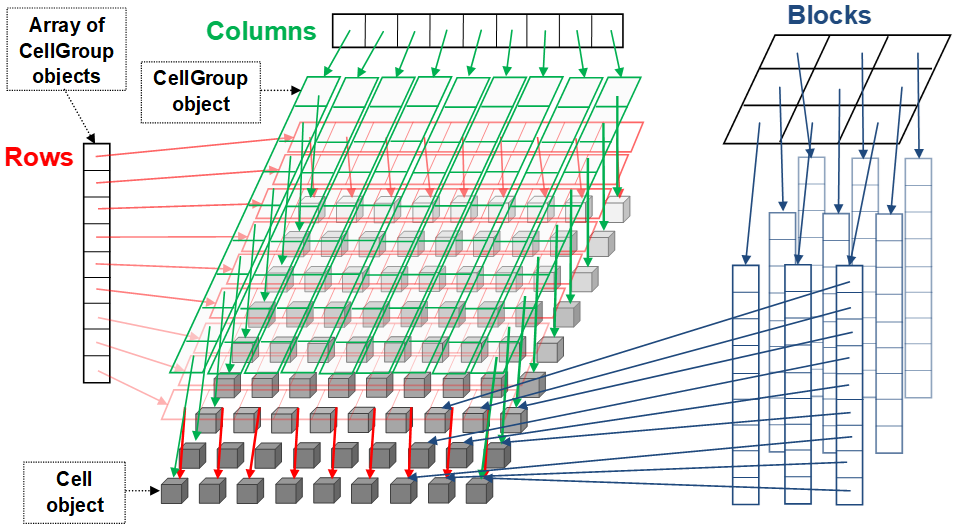
\includegraphics[width=\textwidth]{../README-fig3.png}
            \caption{Top level context index structure}
        \end{figure}

        \subsubsection*{Cell Structure}
            Each cell is a bitmask, representing the possible contents of the actual cell.
            The specification suggests utilizing a flag, stating if a cell was pre-set;
            I have opted not to use this, 
            instead cells are considered solved if any unique bits have been set.
            A cell is stored as a \mintinline{cpp}{char16_t}, 
            2 bytes being the minimum required to store the 9 bit mask.

            \begin{figure}[!h]
                \centering
                \begin{tikzpicture}[start chain=bits going right,
                                    node distance=-0.15mm,
                                    ]
                    
                    \node [on chain=bits] {};
                    \foreach \i in {0,0,0,0,0,0,0}
                        \node [draw, on chain=bits, color=gray] {$\i$};
                    
                    \node [draw, on chain=bits] {$1$};
                    {[start branch=9 going above, text=darkgray] \node [on chain] {$9$};}
                    \node [draw, on chain=bits] {$1$};
                    {[start branch=8 going above, text=darkgray] \node [on chain] {$8$};}
                    \node [draw, on chain=bits] {$0$};
                    {[start branch=7 going above, text=lightgray] \node [on chain] {$7$};}
                    \node [draw, on chain=bits] {$0$};
                    {[start branch=6 going above, text=lightgray] \node [on chain] {$6$};}
                    \node [draw, on chain=bits] {$1$};
                    {[start branch=5 going above, text=darkgray] \node [on chain] {$5$};}
                    \node [draw, on chain=bits] {$1$};
                    {[start branch=4 going above, text=darkgray] \node [on chain] {$4$};}
                    \node [draw, on chain=bits] {$0$};
                    {[start branch=3 going above, text=lightgray] \node [on chain] {$3$};}
                    \node [draw, on chain=bits] {$0$};
                    {[start branch=2 going above, text=lightgray] \node [on chain] {$2$};}
                    \node [draw, on chain=bits] {$0$};
                    {[start branch=1 going above, text=lightgray] \node [on chain] {$1$};}

                    \node [on chain=bits] {};

                    \draw [decoration = {calligraphic brace, raise=9pt, amplitude=10pt, aspect=0.25},
                        decorate, line width=1.5pt] (bits-1) -- (bits-9)
                    node[pos=0.25, above=20pt, black]{\textit{Un-used bits}};

                    \draw [decoration = {calligraphic brace, raise=9pt, amplitude=10pt, mirror},
                        decorate, line width=1.5pt] (bits-8) -- (bits-18)
                    node[pos=0.5, below=20pt, black]{\textit{Masking bits}};

                    \draw [decoration = {brace, raise=20pt, amplitude=5pt},
                        decorate, line width=1.25pt] (bits-12) -- (bits-15)
                    node[pos=0.5, above=25pt, black]{\textit{Possible numbers}};
                \end{tikzpicture}
                \caption{Cell structure with possibilities: \textit{$9$, $8$, $5$, $4$}}
            \end{figure}

            It would have been possible to use an \mintinline{cpp}{enum} of flags,
            however the specific, named constants would have been un-used.

        \begin{listing}[!h]
            \inputminted[gobble=4, firstline=25, lastline=31]{cpp}{../Sudoku/SudokuPuzzle.h}
            \caption{Definition of data structures within Sudoku Solver header}
        \end{listing}

    \subsection*{Loading}
        Due to the how the puzzle files are structured,
        I decided to make use of the previously created \mintinline{cpp}{Grid}
        class, already containing functionality for saving and loading similarly structured files.
        Additional functionality was required, allowing data to be read from and written to
        the grid array.

        \begin{listing}[!h]
            \inputminted[firstline=92]{cpp}{../Sudoku/Grid.cpp}
            \caption{Grid accessors}
        \end{listing}

        Following this existing values had to be loaded into bitmask format,
        and the respective indices created. 
        This can be quickly accomplished through bit-shifting.

        \begin{figure}[H]
            \centering
            \begin{tikzpicture}[node distance=2mm]
                {[start chain=desc going below, node distance=1.8mm]
                    \node[on chain] {\textit{Cell value}};
                    \node[on chain] {\textit{Initial mask state}};
                    \node[on chain] {\textit{Bitshift left by cell value}};
                    \node[on chain] {\textit{Bitshift right once}};
                    \node[on chain] {\textit{Finalized bitmask}};
                }

                {[start chain=0 going below]
                    \node[on chain] at (-2.5,0) {$0$};

                    \node[on chain, draw] {$\textcolor{red}{1}$};
                    {[start branch=00 going left, node distance=-0.15mm, every on chain/.style={draw}]
                        \foreach \i in {0,0,0,0,0,0,0,0}
                            \node[on chain] {$\i$};
                        \node[on chain, color=gray] {$0$};
                    }

                    \node[on chain, draw] {$\textcolor{red}{1}$};
                    {[start branch=01 going left, node distance=-0.15mm, every on chain/.style={draw}]
                        \foreach \i in {0,0,0,0,0,0,0,0}
                            \node[on chain] {$\i$};
                        \node[on chain, color=gray] {$0$};
                    }

                    \node[on chain, draw] {$0$};
                    {[start branch=02 going left, node distance=-0.15mm, every on chain/.style={draw}]
                        \foreach \i in {0,0,0,0,0,0,0,0}
                            \node[on chain] {$\i$};
                        \node[on chain, color=gray] {$0$};
                    }
                }

                {[start chain=1 going below]
                    \node[on chain] at (2.5,0) {$7$};

                    \node[on chain, draw, color=gray] {$0$};
                    {[start branch=10 going right, node distance=-0.15mm, every on chain/.style={draw}]
                        \foreach \i in {0,0,0,0,0,0,0,0,\textcolor{red}{1}}
                            \node[on chain] {$\i$};
                    }

                    \node[on chain, draw, color=gray] {$0$};
                    {[start branch=11 going right, node distance=-0.15mm, every on chain/.style={draw}]
                        \foreach \i in {0,\textcolor{red}{1},0,0,0,0,0,0,0}
                            \node[on chain] {$\i$};
                    }

                    \node[on chain, draw, color=gray] {$0$};
                    {[start branch=11 going right, node distance=-0.15mm, every on chain/.style={draw}]
                        \foreach \i in {0,0,\textcolor{red}{1},0,0,0,0,0,0}
                            \node[on chain] {$\i$};
                    }
                }
            \end{tikzpicture}
            \caption{Creation of cell bitmask}
        \end{figure}

        The result being, all unset cells have false bitmasks, 
        and all pre-set cells mask only for the preset value.
        Assembling the indices however can be accomplished using
        each cells co-ordinates within the 2D array.

        \begin{figure}[!h]
            \centering
            \begin{eqnarray*}
                \text{Cell position:} & & \begin{pmatrix}
                    x & y
                \end{pmatrix}\\
                \text{Column index:} & & \begin{pmatrix}
                    x & y
                \end{pmatrix}\\
                \text{Row index:} & & \begin{pmatrix}
                    y & x
                \end{pmatrix}\\
                \text{Block index:} & &
                \begin{pmatrix}
                    y - (y \bmod 3) + \frac{x - (x \bmod 3)}{3} & 3(y \bmod 3) + (x \bmod 3)
                \end{pmatrix}
            \end{eqnarray*}
            \caption{Methods for obtaining index positions from cell position}
        \end{figure}

        \begin{listing}[H]
            \inputminted[gobble=4, firstline=21, lastline=36]{cpp}{../Sudoku/SudokuPuzzle.cpp}
            \caption{Puzzle load function}
        \end{listing}

    \subsection*{Solving}